%\documentclass[ignorenonframetext,smaller,handout,onlysecheader,sans,fleqn,xcolor=dvipsnames,fleqn,table,stillsansserifmath,stillsansseriftext,stillsansserifsmall,stillsansseriflarge]{beamer}
%\documentclass[ignorenonframetext,onlysecheader,smaller,sans,mathserif,fleqn,handout,xcolor=pdftex,dvipsnames,table]{beamer}
% fontsize=15pt
% for transparencies

% \documentclass[handout]{beamer}
% for handouts

% \documentclass[smaller,handout,sans,xcolor=pdftex,dvipsnames,mathserif,trans,notes=show]{beamer}
% show notes
% \documentclass[smaller,ignorenonframetext,sans,fleqn,mathserif]{beamer}
%\documentclass[smaller,ignorenonframetext,sans,fleqn,xcolor=pdftex,dvipsnames,table,mathserif]{beamer}
% DO NOT show navigation map on top right
\documentclass[smaller,aspectratio=169,ignorenonframetext,compress,sans,fleqn,xcolor=dvipsnames,fleqn,table,stillsansserifmath,stillsansseriftext,stillsansserifsmall,stillsansseriflarge]{beamer} 
%
% SHOW only sec title on top right
%\documentclass[smaller,handout,notes=show,onlysecheader,sans,fleqn,xcolor=dvipsnames,fleqn,table,mathserif]{beamer} 
%\documentclass[ignorenonframetext,smaller,subsecheader,sans,fleqn,xcolor=dvipsnames,fleqn,table,stillsansserifmath,stillsansseriftext,stillsansserifsmall,stillsansseriflarge]{beamer}
%\documentclass[ignorenonframetext,smaller,onlysecheader,sans,fleqn,xcolor=dvipsnames,fleqn,table,stillsansserifmath,stillsansseriftext,stillsansserifsmall,stillsansseriflarge]{beamer}

%try also :
%\documentclass[11pt,fleqn,trans,notes=show,compress]{article}\usepackage{beamerarticle}




\usepackage[english,danish]{babel}
\usepackage[utf8]{inputenc} 
\usepackage[T1]{fontenc}
\usepackage{xcolor}
\usepackage{framed}
%\usepackage[lined]{algorithm2e}
%\usetheme{Odense}
\useoutertheme[height=0pt,width=35pt,hideallsubsections]{sidebar}
\definecolor{myblue}{HTML}{3b5998}
\definecolor{lightblue}{HTML}{8b9dc3}
% files to be included: intro.tex | {commands.tex, beamermysplit.sty}; close.tex

\beamertemplateboldtitlepage
\beamertemplateboldframetitle


%\beamertemplateplaintoc
\beamertemplatenumberedsectiontoc
%\beamertemplatenumberedballsectiontoc

\beamertemplatenavigationsymbolsempty
\beamertemplatetransparentcovered

\setbeamercovered{invisible}
%\renewcommand{\alert}{\textbf}
\setbeamercolor{alerted text}{fg=blue}

%\defbeamertemplate*{background}{Odense theme}{%
%  \hskip0.64\paperwidth%
%  \includegraphics[width=\paperwidth,height=0.88\paperheight,keepaspectratio,trim=0 0 0 -10]{Odense_theme/sdu_seal}%
%}
%
\usesectionheadtemplate
  {\insertsectionhead\hfill}
  {\color{fg!50!bg}\insertsectionhead\hfill}


\mode<article>{\usepackage{fullpage}}
%\mode<article>{\usepackage{SweaveSlides}}
\mode<article>{\renewcommand{\note}[1]{#1}}
%\mode<article>{\newcommand{\code}[1]{\small\texttt{#1}}}

%\mode<presentation|handout>{\usetheme{Odense}}
%\mode<presentation|handout>{\usepackage{SweaveSlides}}

\usepackage{intro}
\usepackage{definitions}
%\usepackage{etex}
%\usepackage{tikz}
%\usetikzlibrary{arrows,decorations.pathmorphing,backgrounds,positioning,fit}


\setbeamercolor{sidebar}{bg=myblue}
\setbeamercolor{structure}{fg=myblue}


\usepackage{animate}

\usepackage{bbding}


\tikzstyle{point}=[circle, draw, fill=black!50,
                        inner sep=0pt, minimum width=4pt]
\newcommand{\plotpoints}{
  \draw node[point] (a) at (1,2) {};% \node[above=2pt of a] {$a$};
  \draw node[point] (b) at (3,0) {};% \node[above=2pt of b] {$b$};
  \draw node[point] (c) at (4,1) {};% \node[above=2pt of c] {$c$};
  \draw node[point] (d) at (7,0) {};% \node[above=2pt of d] {$d$};
  \draw node[point] (e) at (6,2) {};% \node[above=2pt of e] {$e$};
  \draw node[point] (f) at (7,4) {};% \node[above=2pt of f] {$f$};
  \draw node[point] (g) at (3,4) {};% \node[above=2pt of g] {$g$};
}


\graphicspath{{Figures/}}

\title{}


\begin{document}



\begin{frame}[label=secondpage]%%%%%%%%%%%%%%%%%%%%%%%%%%%%%%%%%%%%%%%%%%%%%%%%%%%%%%%%%
  \frametitle{}

%\color{Mahogany}%OliveGreen}
  {\color{myblue}
    \Large\bf        
    DM865 (10 ECTS)\\[1em]
    Heuristikker og Approximationsalgoritmer\\[0.5em]
    {\large [Heuristics and Approximation Algorithms]}\\[2em]
  }

\bigskip
\bigskip
%\bigskip
%\bigskip
\color{black}
\url{dm865.github.io}\\
\vfill
\bigskip
\color{black}
{\small      
Spring semester\\
Lene Monrad Favrholdt \textbullet{} Marco Chiarandini\\lektorer, IMADA\\
%Stefano Gualandi\\
%Researcher, University of Pavia\\
%\url{www-dimat.unipv.it/~gualandi/Home.html}
}


\end{frame}



\begin{frame}%%%%%%%%%%%%%%%%%%%%%%%%%%%%%%%%%%%%%%%%%%%%%%%%%%%%%%%%%%%%%%%%%%

\frametitle{Approximation Algorithms}
\framesubtitle{A $2$-approximation algorithm for TSP}

\begin{columns}[T,onlytextwidth]

  \column{0.5\textwidth}
  \centering
  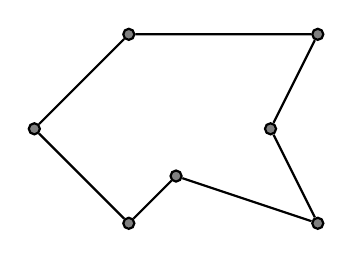
\begin{tikzpicture}[thick,scale=0.6]
%  \draw[very thin,color=gray!50] (0,0) grid (16,9);
  
\plotpoints

\draw (a) -- (b) -- (c) -- (d) -- (e) -- (f) -- (g) -- (a);

  \end{tikzpicture}
  \begin{center}
    $c(TSP)$
  \end{center}
  \column{0.5\textwidth}
  \centering
 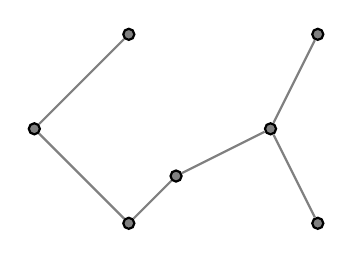
\begin{tikzpicture}[thick,scale=0.6]
%  \draw[very thin,color=gray!50] (0,0) grid (16,9);
  
\plotpoints

\draw[color=gray] (a) -- (b) -- (c) -- (e) -- (d);
    \draw[color=gray] (e) -- (f);
    \draw[color=gray] (a) -- (g);
  \end{tikzpicture}
   \begin{center}
    $c(MST)$
  \end{center}
\end{columns}

\bigskip

\begin{overprint}

\onslide<1|handout:1>
\begin{framed}
Double tree algorithm:
\medskip
\begin{enumerate}
\item $T\leftarrow MST$
\item Double all edges in $T$
\item  $E_{tour} \leftarrow$ Eurler tour
\item $H\leftarrow$ vertices in order of appearance in $E_{tour}$
\end{enumerate}
\end{framed}

\onslide<2-|handout:2>
\begin{center}
\[
c(MST)\leq c(TSP)
\]
\only<3->{
\[
c(H)\leq 2 \cdot c(MST)\leq 2\cdot c(TSP)
\]
}
\end{center}

\end{overprint}

\end{frame}





\begin{frame}%%%%%%%%%%%%%%%%%%%%%%%%%%%%%%%%%%%%%%%%%%%%%%%%%%%%%%%%%%%%%%%%%%

\frametitle{Approximation Algorithms}
\framesubtitle{A $3/2$-approximation algorithm for TSP}

\begin{columns}[T,onlytextwidth]

  \column{0.5\textwidth}
  \centering
  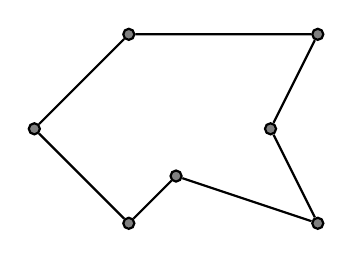
\begin{tikzpicture}[thick,scale=0.6]
%  \draw[very thin,color=gray!50] (0,0) grid (16,9);
  
\plotpoints

\draw (a) -- (b) -- (c) -- (d) -- (e) -- (f) -- (g) -- (a);

  \end{tikzpicture}
  \begin{center}
    $c(TSP)$
  \end{center}
  \column{0.5\textwidth}
  \centering
 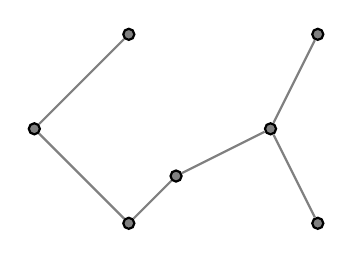
\begin{tikzpicture}[thick,scale=0.6]
%  \draw[very thin,color=gray!50] (0,0) grid (16,9);
  
\plotpoints

\draw[color=gray] (a) -- (b) -- (c) -- (e) -- (d);
    \draw[color=gray] (e) -- (f);
    \draw[color=gray] (a) -- (g);
  \end{tikzpicture}
   \begin{center}
    $c(MST)$
  \end{center}
\end{columns}

\bigskip

\begin{overprint}

\onslide<1|handout:1>
\begin{framed}
  \medskip
  Christofide's algorithm:
\begin{enumerate}
\item $T\leftarrow MST$
\item $M\leftarrow$ minimum perfect matching of odd degree vertices in
  $T$
\item $E_{tour}\leftarrow$ Euler tour in the subgraph $(V,E(T) \cup M)$
\item $H\leftarrow $ vertices in order of appearance in the $E_{tour}$
\end{enumerate}
\end{framed}

\onslide<2-|handout:2>
\begin{center}
\[
c(MST)\leq c(TSP)
\]
\only<3->{
\[
c(H)\leq c(MST) + c(M) \only<4->{\leq c(TSP) +
  \frac{1}{2}c(TSP)} \only<5->{= \frac{3}{2}\cdot c(TSP)}
\]
}
\end{center}

\end{overprint}

\end{frame}



\begin{frame}%%%%%%%%%%%%%%%%%%%%%%%%%%%%%%%%%%%%%%%%%%%%%%%%%%%%%%%%%%%%%%%%%%

  \frametitle{Approximation Algorithms}

  \begin{theorem}[2015]
For $\alpha<\frac{185}{184}$, there does not exist an
$\alpha$-approximation algorithm for the TSP.
  \end{theorem}

  
\end{frame}


\begin{frame}%%%%%%%%%%%%%%%%%%%%%%%%%%%%%%%%%%%%%%%%%%%%%%%%%%%%%%%%%%%%%%%%%%

\frametitle{Local Search}


\begin{columns}[T,onlytextwidth]

\column{0.33\textwidth}
\onslide<1->{
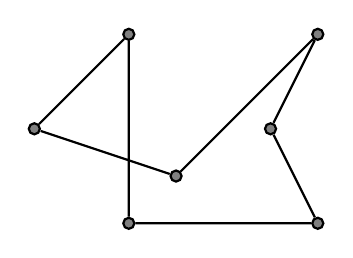
\begin{tikzpicture}[thick,scale=0.6]
\plotpoints
\draw (a) -- (g) -- (b) -- (d) -- (e) -- (f) -- (c) --
    (a);
\end{tikzpicture}
}
\column{0.33\textwidth}
 \onslide<2->{
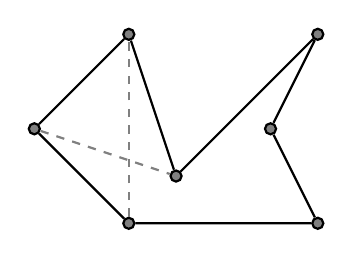
\begin{tikzpicture}[thick,scale=0.6]
\plotpoints
 \draw[] (a) -- (b) -- (d) -- (e) -- (f) -- (c)
    -- (g) -- (a);
    \draw<2>[color=gray,dashed] (a) -- (c);
    \draw<2>[color=gray,dashed] (b) -- (g);
\end{tikzpicture}
}
 \column{0.33\textwidth}
\onslide<4-5>{
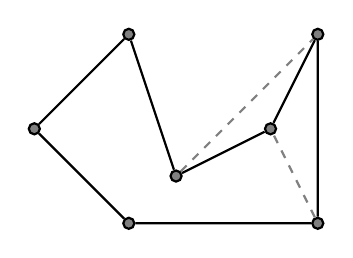
\begin{tikzpicture}[thick,scale=0.6]
\plotpoints
\draw[] (a) -- (b) -- (d) -- (f) -- (e) -- (c)
     -- (g) -- (a);
     \draw<4>[color=gray,dashed] (d) -- (e);
     \draw<4>[color=gray,dashed] (c) -- (f);
\end{tikzpicture}
}
\end{columns}


\end{frame}








\begin{frame}%%%%%%%%%%%%%%%%%%%%%%%%%%%%%%%%%%%%%%%%%%%%%%%%%%%%%%%%%%%%%%%%%%

\frametitle{Metaheuristics}

Accepting worsening changes
\begin{columns}[T,onlytextwidth]
\column{0.33\textwidth}
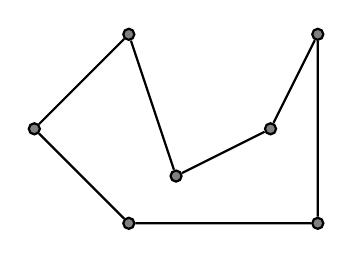
\begin{tikzpicture}[thick,scale=0.6]
 \plotpoints
\draw[] (a) -- (b) -- (d) -- (f) -- (e) -- (c)
     -- (g) -- (a);
\end{tikzpicture}

\onslide<2->{
\column{0.33\textwidth}
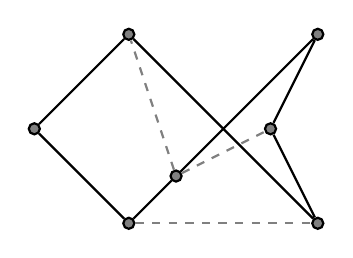
\begin{tikzpicture}[thick,scale=0.6]
 \plotpoints
 \draw[] (a) -- (b) -- (c) -- (f) -- (e) -- (d) -- (g) -- (a);
 \draw<2>[color=gray,dashed] (c) -- (g);
 \draw<2>[color=gray,dashed] (b) -- (d);
 \draw<2>[color=gray,dashed] (c) -- (e);
\end{tikzpicture}
}

\onslide<4->{
\column{0.33\textwidth}
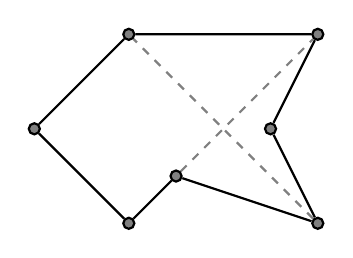
\begin{tikzpicture}[thick,scale=0.6]
  \plotpoints
  \draw[] (a) -- (b) -- (c) -- (d) -- (e) -- (f) -- (g) -- (a);
 \draw<4>[color=gray,dashed] (d) -- (g);
 \draw<4>[color=gray,dashed] (c) -- (f);
\end{tikzpicture}
}

\end{columns}
  
\bigskip
\bigskip

\onslide<6->{
Trying different changes
\begin{columns}[T,onlytextwidth]
\pause
\column{0.33\textwidth}
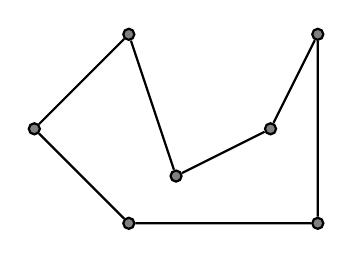
\begin{tikzpicture}[thick,scale=0.6]
 \plotpoints
\draw[] (a) -- (b) -- (d) -- (f) -- (e) -- (c)
-- (g) -- (a);
\end{tikzpicture}
}

\column{0.33\textwidth}
\onslide<8->{
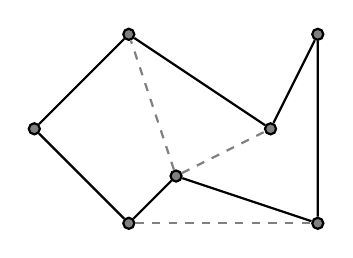
\begin{tikzpicture}[thick,scale=0.6]
 \plotpoints
  \draw[] (a) -- (b) -- (c) -- (d) -- (f) -- (e) -- (g) -- (a);
 \draw<8>[color=gray,dashed] (b) -- (d);
 \draw<8>[color=gray,dashed] (c) -- (g);
  \draw<8>[color=gray,dashed] (c) -- (e);
\end{tikzpicture}
}

\column{0.33\textwidth}

\onslide<10-11>{
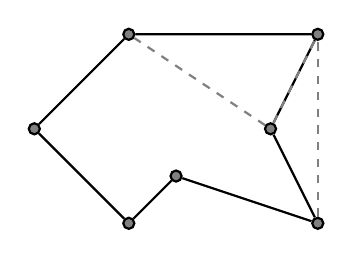
\begin{tikzpicture}[thick,scale=0.6]
 \plotpoints
 \draw[] (a) -- (b) -- (c) -- (d) -- (e) -- (f) -- (g) -- (a);
  \draw<10>[color=gray,dashed] (e) -- (f);
 \draw<10>[color=gray,dashed] (e) -- (g);
  \draw<10>[color=gray,dashed] (d) -- (f);
\end{tikzpicture}
}
\end{columns}


\end{frame}




\begin{frame}%%%%%%%%%%%%%%%%%%%%%%%%%%%%%%%%%%%%%%%%%%%%%%%%%%%%%%%%%%%%%%%%%%

\frametitle{Contents}

\begin{table}
  \centering
\begin{tabular}{l|p{4.5cm}p{4.5cm}}
&Apporx Algorithms&Local Search + Metaheuristics\\
\hline
  Set Cover&&\\
Satisfiability&&\\
Traveling Salesman&&\\
Scheduling&&\\
Knapsack&&\\
Bin packing&&
\end{tabular}
\end{table}
  
\end{frame}




\frame{%%%%%%%%%%%%%%%%%%%%%%%%%%%%%%%%%%%%%%%%%%%%%%%%%%%%%%%%%%%%%%%%%%%%%

\frametitle{Course Formalities}

\begin{tabular}{ll}
%\hline
\parbox[t]{0.18\textwidth}{\alert{Prerequisites:}} &\begin{minipage}[t]{0.72\textwidth}
\begin{itemize}
\item[\CheckmarkBold] Programming (DM502, DM503, DM550)
\item[\CheckmarkBold] Algorithms and Datastructures (DM507)
\item[\color{gray}\Checkmark] Complexity and Computability (DM508, DM553)
\item[\color{gray}\Checkmark] Linear and Integer Programming (DM559, DM545, DM554, DM871)
\end{itemize}
\end{minipage}\\
&\\
%\hline
\parbox[t]{0.2\textwidth}{\alert{Credits:}} &\begin{minipage}[t]{0.7\textwidth}
\smallskip
10 ECTS
\end{minipage}\\
&\\
%\hline
\parbox[t]{0.2\textwidth}{\alert{Language:}} &\begin{minipage}[t]{0.7\textwidth}
\smallskip
English or Danish
\end{minipage}\\
&\\
%\hline
\parbox[t]{0.2\textwidth}{\alert{Classes:}}& 
\begin{minipage}[t]{0.7\textwidth}
\smallskip
intro: $2h\times 20$; training: $2h\times 15$ 
\end{minipage}\\
&\\
%\hline
\parbox[t]{0.2\textwidth}{\alert{Material:}}& 
\begin{minipage}[t]{0.7\textwidth}
\smallskip
slides + text book + articles + starting code
\end{minipage}\\
&\\
%\hline
%Exercises: 14h (but some will be taken up by the project)
\end{tabular}
}






\begin{frame}%%%%%%%%%%%%%%%%%%%%%%%%%%%%%%%%%%%%%%%%%%%%%%%%%%%%%%%%%%%%%%%%%%
  \frametitle{Assessment (10 ECTS)}


\medskip

\begin{itemize}

\itemsep=3ex

\item  Two practical project assignments passed/failed with internal censor by
  the teacher\\
  (include programming in Python)

\item Oral exam based on:
  \begin{itemize}

  \item the theoretical part
  \item two practical assignments
  \end{itemize}
Grading by the Danish 7-mark
scale with external examiner. Exam aids allowed.
\end{itemize}

\end{frame}




\againframe{secondpage}



\end{document}


